\documentclass[12pt, a4paper]{article}

\usepackage{amsmath}
\usepackage{amsfonts}
\usepackage{amssymb}
\usepackage{graphicx}
\usepackage{float}
\usepackage{listings}
\usepackage{rotating}
\usepackage{tikz}
\pdfgentounicode=1
\pdfmapline{+cyberb@Unicode@  <cyberbit.ttf}

\begin{document}

\title{MozaIt}
\author{P. Baillehache}
\date{\today}
\maketitle

\tableofcontents

\section*{Introduction}

MozaIt is a C library to generate a dot representation of a picture. It is also a web application to use this library through a webpage.\\

The representation is made by packing circles of fixed sizes, starting with the biggest and going down the smallest, at location where the difference between average color inside the circles and the color at the center of the circle is below a threshold. The threshold and the range of sizes are defined by the user. The sizes are constraint to powers of $\varphi$ (the golden ratio). Finally a margin parameter allows the user to control the minimum spacing between circles. As a background, the algorithm allows the user to choose a color, or to let the algorithm fill in with the average of the colors on the whole source image.\\

The web application allows the user to use the software in a straightforward way. After downloading a source image and selecting the value of parameters, the user gets the result image in one click. The web application limits the size of source images to less than 500x500 pixels to avoid very long computation time and load on the server. Images are deleted when the user leaves the page to protect his privacy.\\

\section{C}

\subsection{Interface}

\begin{scriptsize}
\begin{ttfamily}
\begin{lstlisting}
// ============ MOZAIT.H ================

#ifndef MOZAIT_H
#define MOZAIT_H

// ================= Include =================

#include <stdlib.h>
#include <stdio.h>
#include <math.h>
#include <string.h>
#include <stdbool.h>
#include "gset.h"
#include "tgapaint.h"

// ================= Define ==================


// ================= Data structures ===================

// Types of background
typedef enum MozaItBackground {
  // Solid color
  MozaItBackgroundSolid,
  // Average color
  MozaItBackgroundAvg
} MozaItBackground;

// MozaIt options
typedef struct MozaItOpt {
  // Orders defining the size min and max of the tiles
  // size = pow(golden ratio, order)
  int _orders[2];
  // Margin around the tile, in pixel
  float _margin;
  // Threshold in [0.0, 1.0] (0.0: strict, 1.0: loose)
  float _threshold;
  // Type of background
  MozaItBackground _typeBg;
  // Background color in case of solid background
  unsigned char _rgbaBg[4];
} MozaItOpt;

// MozaIt
typedef struct MozaIt {
  // MozaIt options
  MozaItOpt _option;
} MozaIt;

// ================ Functions declaration ====================

// Create a new MozaIt with default options' value:
// _orders = {1, 10}
// _margin = 2
// _threshold = sqrt(0.1)
// _typeBg = MozaItBackgroundAvg
// Return NULL if we couldn't create the MozaIt
MozaIt* MozaItCreate(void);

// Free the memory used by a MozaIt
// Do nothing if arguments are invalid
void MozaItFree(MozaIt **moz);

// Set the min and max orders (in [0, 12])
// Do nothing if arguments are invalid
void MozaItSetMinMaxOrder(MozaIt *moz, int *orders);

// Set the margin
// Do nothing if arguents are invalid
void MozaItSetMargin(MozaIt *moz, float margin);

// Set the threshold
// Do nothing if arguents are invalid
void MozaItSetThreshold(MozaIt *moz, float threshold);

// Set the background type to solid
// Do nothing if arguents are invalid
void MozaItSetSolidBackground(MozaIt *moz, unsigned char *rgba);

// Set the background type to average
// Do nothing if arguents are invalid
void MozaItSetAvgBackground(MozaIt *moz);

// Process the TGA 'src' and return the resulting TGA
// Return NULL if arguments are invalid or couldn't
// process the image
TGA* MozaItProcess(MozaIt *moz, TGA *src);

#endif
\end{lstlisting}
\end{ttfamily}
\end{scriptsize}

\subsection{Code}

\begin{scriptsize}
\begin{ttfamily}
\begin{lstlisting}
// ============ MOZAIT.C ================

// ================= Include ==================

#include "mozait.h"

// ================= Define ==================

#define rnd() (float)(rand())/(float)(RAND_MAX)
#define MOZAIT_GOLDENRATIO 1.61803

// ================ Functions declaration ====================

// Check if a tile of siwe 'size' centered at 'pos' is possible for 
// image 'src' and mask 'mask'
// Return true if possible, false else
bool MozaItCheckPos(MozaIt *moz, VecShort *pos, float size, 
  bool *mask, TGA *src);

// Draw one tile of siwe 'siwe' centered at 'pos' in TGA 'tga' and update
// the mask 'mask'
void MozaItDrawTile(MozaIt *moz, VecShort *pos, float size, bool *mask, 
  TGA *src, TGA *tga);
  
// ================ Functions implementation ====================

// Create a new MozaIt with default options' value:
// _orders = {1, 10}
// _margin = 2
// _threshold = 0.1
// _typeBg = MozaItBackgroundAvg
// Return NULL if we couldn't create the MozaIt
MozaIt* MozaItCreate(void) {
  // Allocate memory
  MozaIt *ret = (MozaIt*)malloc(sizeof(MozaIt));
  // If we could allocate memory
  if (ret != NULL) {
    // Set the default options
    ret->_option._orders[0] = 1;
    ret->_option._orders[1] = 9;
    ret->_option._margin = 2.0;
    ret->_option._threshold = sqrt(0.1);
    ret->_option._typeBg = MozaItBackgroundAvg;
    ret->_option._rgbaBg[0] = 255;
    ret->_option._rgbaBg[1] = 255;
    ret->_option._rgbaBg[2] = 255;
    ret->_option._rgbaBg[3] = 255;
  }
  // Return the MozaIt
  return ret;
}

// Free the memory used by a MozaIt
// Do nothing if arguments are invalid
void MozaItFree(MozaIt **moz) {
  // Check the arguments
  if (moz == NULL || *moz == NULL)
    return;
  // Free memory
  free(*moz);
  *moz = NULL;
}

// Set the min and max orders (in [0, 12])
// Do nothing if arguents are invalid
void MozaItSetMinMaxOrder(MozaIt *moz, int *orders) {
  // Check the arguments
  if (moz == NULL || orders == NULL || orders[0] > orders[1] || 
    orders[0] < 0 || orders[1] > 12)
    return;
  // Set the dimensions
  for (int iDim = 0; iDim < 2; ++iDim)
    moz->_option._orders[iDim] = orders[iDim];
}

// Set the margin
// Do nothing if arguents are invalid
void MozaItSetMargin(MozaIt *moz, float margin) {
  // Check the arguments
  if (moz == NULL || margin < 0.0)
    return;
  // Set the margin
  moz->_option._margin = margin;
}

// Set the threshold
// Do nothing if arguents are invalid
void MozaItSetThreshold(MozaIt *moz, float threshold) {
  // Check the arguments
  if (moz == NULL || threshold < 0.0 || threshold > 1.0)
    return;
  // Set the threshold
  moz->_option._threshold = threshold;
}

// Set the background type to solid
// Do nothing if arguents are invalid
void MozaItSetSolidBackground(MozaIt *moz, unsigned char *rgba) {
  // Check the arguments
  if (moz == NULL || rgba == NULL)
    return;
  // Set the background
  moz->_option._typeBg = MozaItBackgroundSolid;
  for (int iRGB = 0; iRGB < 4; ++iRGB)
    moz->_option._rgbaBg[iRGB] = rgba[iRGB];
}

// Set the background type to average
// Do nothing if arguents are invalid
void MozaItSetAvgBackground(MozaIt *moz) {
  // Check the arguments
  if (moz == NULL)
    return;
  // Set the background
  moz->_option._typeBg = MozaItBackgroundAvg;
}

// Process the TGA 'src' and return the resulting TGA
// Return NULL if arguments are invalid or couldn't
// process the image
TGA* MozaItProcess(MozaIt *moz, TGA *src) {
  // Check the arguments
  if (moz == NULL || src == NULL)
    return NULL;
  // Declare a variable to memorize the dimensions of the TGA
  VecShort *dim = VecShortCreate(2);
  if (dim == NULL)
    return NULL;
  VecSet(dim, 0, src->_header->_width);
  VecSet(dim, 1, src->_header->_height);
  // Declare a variable to memorize the background color
  TGAPixel *pixel = NULL;
  // Set the background color
  if (moz->_option._typeBg == MozaItBackgroundSolid) {
    pixel = TGAGetWhitePixel();
    if (pixel != NULL)
      for (int iRGB = 0; iRGB < 4; ++iRGB)
        pixel->_rgba[iRGB] = moz->_option._rgbaBg[iRGB];
  } else if (moz->_option._typeBg == MozaItBackgroundAvg) {
    pixel = TGAGetAverageColor(src);
  } else {
    pixel = TGAGetWhitePixel();
  }
  // If we coudln't create the pixel for the background color
  if (pixel == NULL) {
    // Stop here
    VecFree(&dim);
    return NULL;
  }
  // Create the result TGA
  TGA *tga = TGACreate(dim, pixel); 
  // If we couldn't create the tga
  if (tga == NULL) {
    // Stop here
    VecFree(&dim);
    TGAPixelFree(&pixel);
    return NULL;
  }
  // Declare a variable to memorize pixels painted
  bool *mask = (bool*)malloc(sizeof(bool) * VecGet(dim, 0) * VecGet(dim, 1));
  // If we couldn't allocate memory for the mask
  if (mask == NULL) {
    // Free memory
    TGAPixelFree(&pixel);
    TGAFree(&tga);
    VecFree(&dim);
    // Stop here
    return NULL;
  }
  // Initialize the mask
  for (int i = VecGet(dim, 0) * VecGet(dim, 1); i--;)
    mask[i] = false;
  // Declare a pencil to paint on the result TGA
  TGAPencil *pen = TGAGetPencil();
  // If we couldn't allocate memory for the pen
  if (pen == NULL) {
    // Free memory
    TGAPixelFree(&pixel);
    TGAFree(&tga);
    VecFree(&dim);
    // Stop here
    return NULL; 
  }
  // Declare a variable to memorize the min and max sizes of the tiles
  float sizes[2];
  for (int iSize = 0; iSize < 2; ++iSize)
    sizes[iSize] = pow(MOZAIT_GOLDENRATIO, moz->_option._orders[iSize]);
  // Declare a variable to memorize the order in which we move through
  // the image (abciss first or ordinate first)
  // By giving priority to the longest axis it speed up the process
  // thanks to the skipping of pixels in intersection when we achieve
  // a tile placement
  int axis[2];
  if (VecGet(dim, 0) > VecGet(dim, 1)) {
    axis[0] = 0;
    axis[1] = 1;
  } else {
    axis[0] = 1;
    axis[1] = 0;
  }
  // Fill the TGA starting with big tiles down to smallest tiles
  for (float size = sizes[1]; size >= sizes[0]; 
    size /= MOZAIT_GOLDENRATIO) {
    // Declare a variable to memorize the number of tiles found
    int nbTile = 0;
    // Declare a variable to memorize the size of the tile with margin
    short r = (short)floor(size + moz->_option._margin);
    // For each possible position of this tile
    // Step by 2 to speed up the process without decreasing the quality
    // of the result
    VecShort *pos = VecShortCreate(2);
    if (pos == NULL) {
      // Free memory
      TGAPixelFree(&pixel);
      TGAFree(&tga);
      VecFree(&dim);
      TGAPencilFree(&pen);
      // Stop here
      return NULL; 
    }
    for (VecSet(pos, axis[1], r); 
      VecGet(pos, axis[1]) <= VecGet(dim, axis[1]) - r; 
      VecSet(pos, axis[1], VecGet(pos, axis[1]) + 2)) { 
      for (VecSet(pos, axis[0], r); 
        VecGet(pos, axis[0]) <= VecGet(dim, axis[0]) - r; 
        VecSet(pos, axis[0], VecGet(pos, axis[0]) + 2)) { 
        // Get the index of this position
        int index = VecGet(pos, 1) * src->_header->_width + 
          VecGet(pos, 0);
        // If this position is free
        if (mask[index] == false && MozaItCheckPos(moz, pos, size, mask, src) == true) {
          // Draw the tile
          MozaItDrawTile(moz, pos, size, mask, src, tga);
          // Update the number of tiles
          ++nbTile;
          // Skip the next pixels which are in intersection with the tile
          VecSet(pos, axis[0], VecGet(pos, axis[0]) + 
            (short)floor(size * 2));
        }
      }
    }
    VecFree(&pos);
  }
  // Free memory
  TGAPixelFree(&pixel);
  VecFree(&dim);
  free(mask);
  mask = NULL;
  TGAPencilFree(&pen);
  // Return the result TGA
  return tga;
}

// Check if a tile of radius 'size' centered at 'pos' is possible for 
// image 'src' and mask 'mask'
// Return true if possible, false else
bool MozaItCheckPos(MozaIt *moz, VecShort *pos, float size, bool *mask, 
  TGA *src) { 
  // Declare a variable to memorize the size of the square covering the 
  // tile
  short r = (short)floor(size + moz->_option._margin);
  // Declare variables to calculate the average delta of color
  float avg[3] = {0.0};
  float sum = 0.0;
  // Declare a variable to memorize if the tile touch the mask
  bool maskOk = true;
  // Get the pixel in the source image at center of tile
  TGAPixel *pixelSrc = TGAGetPix(src, pos);
  // For each pixel in the square covering the tile
  VecShort *p = VecShortCreate(2);
  if (p == NULL)
    return false;
  for (VecSet(p, 0, VecGet(pos, 0) - r); 
    VecGet(p, 0) <= VecGet(pos, 0) + r && maskOk == true; 
    VecSet(p, 0, VecGet(p, 0) + 1)) {
    for (VecSet(p, 1, VecGet(pos, 1) - r); 
      VecGet(p, 1) <= VecGet(pos, 1) + r && maskOk == true; 
      VecSet(p, 1, VecGet(p, 1) + 1)) {
      // Get the index of this position
      int index = VecGet(p, 1) * src->_header->_width + VecGet(p, 0);
      // Calculate the distance to the center
      float d = sqrt(pow(VecGet(pos, 0) - VecGet(p, 0), 2.0) + pow(VecGet(pos, 1) - VecGet(p, 1), 2.0));
      // If this pos is in the margin
      if (d <= r) {
        // Check the mask
        if (mask[index] == true)
          maskOk = false;
        // Else, if this pos is in the tile
        else if (d <= size) {
          // Get the pixel in the source image at current pos
          TGAPixel *pixel = TGAGetPix(src, p);
          // Update the average delta of color
          // The delta is weighted with the square of the distance
          // to counteract the fact that as the circle get bigger 
          // delta of color of one pixel gets relatively less and
          // less significant 
          sum += d * d;
          for (int iRGB = 3; iRGB--;)
            avg[iRGB] += 
              fabs((float)(pixel->_rgba[iRGB]) - 
              (float)(pixelSrc->_rgba[iRGB])) / 255.0 *
              d * d;
        }
      }
    }
  }
  VecFree(&p);
  // Complete the calculation of the average delta of color
  for (int iRGB = 0; iRGB < 3; ++iRGB)
    avg[iRGB] /= sum;
  // Calculate the distance of the average delta of color in the tile
  float dColor = sqrt(pow(avg[0], 2.0) + pow(avg[1], 2.0) + 
    pow(avg[2], 2.0));
  // If the tile doesn't touch the mask and the average color respects
  // the threshold
  if (maskOk == true && dColor <= pow(moz->_option._threshold, 2.0)) {
    return true;
  // Else, the tile touches the mask or the average color doesn't respect
  // the threshold
  } else {
    return false;
  }
}

// Draw one tile of siwe 'siwe' centered at 'pos' in TGA 'tga' and update
// the mask 'mask'
void MozaItDrawTile(MozaIt *moz, VecShort *pos, float size, bool *mask, 
  TGA *src, TGA *tga) {
  // Declare a variable to memorize the size of the square covering the 
  // tile
  short r = (short)floor(size);
  // Get the pixel in the source image at center of tile
  TGAPixel *pixel = TGAGetPix(src, pos);
  // For each pixel in the square covering the tile
  VecShort *p = VecShortCreate(2);
  for (VecSet(p, 0, VecGet(pos, 0) - r); 
    VecGet(p, 0) <= VecGet(pos, 0) + r; 
    VecSet(p, 0, VecGet(p, 0) + 1)) {
    for (VecSet(p, 1, VecGet(pos, 1) - r); 
      VecGet(p, 1) <= VecGet(pos, 1) + r; 
      VecSet(p, 1, VecGet(p, 1) + 1)) {
      // Get the index of this position
      int index = VecGet(p, 1) * src->_header->_width + VecGet(p, 0);
      // Calculate the distance to the center
      float d = sqrt(pow(VecGet(pos, 0) - VecGet(p, 0), 2.0) + 
        pow(VecGet(pos, 1) - VecGet(p, 1), 2.0));
      // If this pos is in the tile
      if (d <= size) {
        // Get the pixel in the result image at current pos
        TGAPixel *pixelOut = TGAGetPix(tga, p);
        // Update the color
        for (int iRGB = 3; iRGB--;)
          pixelOut->_rgba[iRGB] = pixel->_rgba[iRGB];
        // Update the mask
        mask[index] = true;
      }
    }
  }
}
\end{lstlisting}
\end{ttfamily}
\end{scriptsize}

\subsection{Makefile}

\begin{scriptsize}
\begin{ttfamily}
\begin{lstlisting}
OPTIONS_DEBUG=-ggdb -g3 -Wall
OPTIONS_RELEASE=-O3 
OPTIONS=$(OPTIONS_RELEASE)
INCPATH=/home/bayashi/Coding/Include
LIBPATH=/home/bayashi/Coding/Include

all : mozait

mozait: main.o mozait.o Makefile $(LIBPATH)/tgapaint.o $(LIBPATH)/gset.o $(LIBPATH)/pbmath.o $(LIBPATH)/bcurve.o
	gcc  $(OPTIONS) main.o $(LIBPATH)/tgapaint.o $(LIBPATH)/gset.o $(LIBPATH)/pbmath.o $(LIBPATH)/bcurve.o mozait.o -o mozait -lm

main.o : main.c mozait.h Makefile
	gcc $(OPTIONS) -I$(INCPATH) -c main.c

mozait.o : mozait.c mozait.h $(INCPATH)/tgapaint.h $(INCPATH)/gset.h Makefile
	gcc $(OPTIONS) -I$(INCPATH) -c mozait.c

clean : 
	rm -rf *.o mozait

test :
	./mozait test03.tga out.tga

valgrind :
	valgrind -v --track-origins=yes --leak-check=full --gen-suppressions=yes --show-leak-kinds=all ./mozait test01.tga out.tga
\end{lstlisting}
\end{ttfamily}
\end{scriptsize}

\subsection{Usage}

\begin{scriptsize}
\begin{ttfamily}
\begin{lstlisting}
// ============ MAIN.C ================

// ================= Include ==================

#include <stdlib.h>
#include <stdio.h>
#include <time.h>
#include <string.h>
#include "mozait.h"

// ================= Main function ==================

int main(int argc, char **argv) {
  // Create the MozaIt
  MozaIt *moz = MozaItCreate();
  // If we couldn't create the MozaIt
  if (moz == NULL) {
    // Display a message and stop
    fprintf(stdout, "Couldn't create the MozaIt\n");
    return 1;
  }
  // Declare variables to process the arguments
  char *fileNameIn = NULL;
  char *fileNameOut = NULL;
  // Declare a variable to memorize the usage
  char *usage = "Usage: mozait <input.tga> <output.tga> \
[-order <min> <max> (in [0,12])] \
[-margin <margin> (in pixel)] \
[-threshold <threshold> (in [0.0,1.0]) \
[solid <r> <g> <b> <a> (in [0, 255]) \
[-average]\n";
  // If the number of arguments is invalid
  if (argc < 3) {
    // Display the usage
    fprintf(stdout, "%s", usage);
    // Free memory
    MozaItFree(&moz);
    // Stop here
    return 2;
  // Else, the number of argument is valid
  } else {
    // Process the arguments
    fileNameIn = argv[1];
    fileNameOut = argv[2];
    // For each optional argument
    for (int iArg = 3; iArg < argc; ++iArg) {
      if (strcmp(argv[iArg], "-order") == 0 && iArg + 2 < argc) {
        int o[2];
        o[0] = atoi(argv[iArg + 1]);
        o[1] = atoi(argv[iArg + 2]);
        MozaItSetMinMaxOrder(moz, o);
        iArg += 2;
      } else if (strcmp(argv[iArg], "-margin") == 0 && iArg + 1 < argc) {
        float m = atof(argv[iArg + 1]);
        MozaItSetMargin(moz, m);
        iArg += 1;
      } else if (strcmp(argv[iArg], "-threshold") == 0 && 
        iArg + 1 < argc) {
        float t = atof(argv[iArg + 1]);
        MozaItSetThreshold(moz, t);
        iArg += 1;
      } else if (strcmp(argv[iArg], "-solid") == 0 && iArg + 4 < argc) {
        unsigned char r[4];
        r[0] = atoi(argv[iArg + 1]);
        r[1] = atoi(argv[iArg + 2]);
        r[2] = atoi(argv[iArg + 3]);
        r[3] = atoi(argv[iArg + 4]);
        MozaItSetSolidBackground(moz, r);
        iArg += 4;
      } else if (strcmp(argv[iArg], "-average") == 0) {
        MozaItSetAvgBackground(moz);
      } else {
        // Display the usage
        fprintf(stdout, "%s", usage);
        // Free memory
        MozaItFree(&moz);
        // Stop here
        return 3;
      }
    }
  }
  // If the user gave proper arguments
  if (fileNameIn != NULL && fileNameOut != NULL) {
    // Open the input TGA
    TGA *tgaIn = NULL;
    int ret = TGALoad(&tgaIn, fileNameIn);
    // If we couldn't load the input TGA
    if (ret != 0) {
      // Display a message
      fprintf(stdout, "Couldn't load %s (%d)\n", fileNameIn, ret);
      // Free memory
      MozaItFree(&moz);
      // Stop here
      return 4;
    }
    // Check the size of the source image
    /*if (tgaIn->_header->_width > 500 || tgaIn->_header->_height > 500) {
      // Display a message
      fprintf(stdout, "Source image too big\n");
      // Free memory
      MozaItFree(&moz);
      // Stop here
      return 7;
    }*/
    // Process the input TGA
    TGA *tgaOut = MozaItProcess(moz, tgaIn);
    // If we couldn't process the TGA
    if (tgaOut == NULL) {
      // Display a message
      fprintf(stdout, "Couldn't process the TGA\n");
      // Free memory
      TGAFree(&tgaIn);
      MozaItFree(&moz);
      // Stop here
      return 5;
    }
    // Save the output TGA
    ret = TGASave(tgaOut, fileNameOut);
    // If we couldn't load the input TGA
    if (ret != 0) {
      // Display a message
      fprintf(stdout, "Couldn't save %s (%d)\n", fileNameOut, ret);
      // Free memory
      TGAFree(&tgaIn);
      MozaItFree(&moz);
      // Stop here
      return 6;
    }
    // Free memory
    TGAFree(&tgaIn);
    TGAFree(&tgaOut);
  }
  // Free memory
  MozaItFree(&moz);
  // Return the success code
  return 0;
}
\end{lstlisting}
\end{ttfamily}
\end{scriptsize}

\section{Web}

\subsection{Resources}

List of files 

\begin{scriptsize}
\begin{ttfamily}
\begin{lstlisting}
./index.php : main web page
./mozait.css : CSS
./mozait.js : JavaScript functions
./upload.php : interface for HTTP Request for uploading and deleting images
./requestPicture.php : interface for HTTP Request for executing the binary
./mozait : binary of MozaIt
./jquery.min.js : JQuery library
./animate.css : Animate library
Img/close.gif : close button for the setting panel
Img/mozait.ico : icon of the webpage
Img/wait.gif : animated GIF used during long operation
Src/ : folder containing the source images
Res/ : folder containing the result images
\end{lstlisting}
\end{ttfamily}
\end{scriptsize}

\begin{center}
\begin{figure}[H]
\centering

\includegraphics[width=3cm]{./close.png}\\
close.gif
\end{figure}
\end{center}

\begin{center}
\begin{figure}[H]
\centering

\includegraphics[width=3cm]{./mozait.png}\\
mozait.ico
\end{figure}
\end{center}

\begin{center}
\begin{figure}[H]
\centering

\includegraphics[width=3cm]{./wait.png}\\
wait.gif
\end{figure}
\end{center}

\subsection{index.php}

\begin{scriptsize}
\begin{ttfamily}
\begin{lstlisting}
<?php 
  // ------------------ index.php --------------------->
  // Start the PHP session
  session_start();

  // Ensure no message will interfere with output
  ini_set('display_errors', 'Off');
  error_reporting(0);

  // Turn on display of errors and warning for debug
  /*ini_set('display_errors', 'On');
  error_reporting(E_ALL ^ E_WARNING);
  error_reporting(E_ALL | E_STRICT);*/

?>
<!DOCTYPE html>
<html>
  <head>

    <!-- Meta -->
    <meta content="text/html; charset=UTF-8;">
    <meta name="viewport" 
      content="width=device-width, initial-scale=1, maximum-scale=1">
    <meta name="description" content="MozaIt! " />
    <meta name="keywords" content="mozait, mozaic, painting" />
      
    <!-- Icon -->
    <link rel="icon" type="image/x-icon" 
      href="./Img/mozait.ico" />

    <!-- Include the CSS files -->
    <link href = "./animate.css" 
      rel = "stylesheet" type = "text/css">
    <link href = "./mozait.css" 
      rel = "stylesheet" type = "text/css"> 

    <!-- Include the JS files -->
    <script charset = "UTF-8" src = "./jquery.min.js"></script>
    <script charset = "UTF-8" src = "./mozait.js"></script>

    <title>MozaIt!</title>
  </head>
  <body onload = <?php echo "'BodyOnLoad(" . date("YmdHis") . ");'" ?>>
    <!-- Main div -->
    <div id = "divMain">
      
      <!-- Title div -->
      <div id = "divTitle">
        MozaIt!<br>
        <div id = "divSubTitle">
          - Transform your pictures into mozaic of dots -
        </div>
      </div>
      
      <!-- Main div -->
      <div id = "divBoard">
        <div id = "divInputImg" class = "divTool">
          Source image:<br><br>
          <div id = "divInfoSrc">
            Click below to select a source image<br>
            (.jpg, RGB, less than 500x500 pixels only !).<br>
            The image will be displayed after upload is complete.<br>
            <form id = "formSrcImg" action = "" method = "post" 
            enctype = "multipart/form-data">
              <input type = "file" name = "inpSrcImg" 
              id = "inpSrcImg" style = "width:250px;" 
              onChange = "SelectSrcImg();">
            </form>
            <img id = "imgWaitSrc" src = "./Img/wait.gif" 
              style = "display:none;">
          </div>
          <img id = "imgSrc">
        </div>
        <div id = "divOutputImg" class = "divTool">
          Result image:<br><br>
          <div id = "divInfoOut">
            Click on the "MozaIt!" button below to display the result 
            image. <br>
            It may takes a few seconds to a few minutes, please be 
            patient.<br>
            If you're not satisfied with the result, experiment
            with the settings below.
          </div>
          <div id = "divMsgOut"></div>
          <img id = "imgWait" src = "./Img/wait.gif" 
            style = "display:none;">
          <img id = "imgOut">
        </div>
      </div>
      
      <!-- Cmd div -->
      <div id = "divCmd">
        <input type = "button" value = "MozaIt!" 
          onclick = "Process();">
        <input type = "button" value = "Settings" 
          onclick = "ShowSettings();">
        <input type = "button" value = "Change source" 
          id = "btnChangeSrc" onclick = "ChangeSource();" 
          style = "display: none;">
      </div>

      <!-- footer div -->
      <div id = "divFooter">
        Copyright <a href="mailto:Pascal@BayashiInJapan.net">
            P. Baillehache
        </a>, 2017.<br>
        Your images are stored on the server only for the time they are
        processed.<br>They are automatically deleted once you leave 
        this page.
      </div>

    </div>

    <!-- Setting div -->
    <div id = "divSettings">
      <div id = "divSettingsContent">
        <img src = "./Img/close.gif" id = "imgSettingsClose"
          onclick = "HideSettings();">
        <div id = "divSettingsTitle">- Settings -</div>
        <div class = "divOneSetting">
          Size of smallest dot (<span id = "spanMinOrder"></span>): 
          <input type = "range" min = "0" max = "12" value = "1"
            id = "rngMinOrder" class = "rng" onChange = "SetMinOrder();">
        </div>
        <div class = "divOneSetting">
          Size of largest dot (<span id = "spanMaxOrder"></span>): 
          <input type = "range" min = "0" max = "12" value = "10"
            id = "rngMaxOrder" class = "rng" onChange = "SetMaxOrder();">
        </div>
        <div class = "divOneSetting">
          Blurriness (<span id = "spanThreshold"></span>): 
          <input type = "range" min = "0.0" max = "1.0" value = "0.3"
            step = "0.01" id = "rngThreshold" class = "rng"  
            onChange = "SetThreshold();">
        </div>
        <div class = "divOneSetting">
          Margin between dots (<span id = "spanMargin"></span>): 
          <input type = "range" min = "0" max = "20" value = "2"
            id = "rngMargin" class = "rng" onChange = "SetMargin();">
        </div>
      </div>
    </div>
      
  </body>

</html>
\end{lstlisting}
\end{ttfamily}
\end{scriptsize}

\subsection{mozait.css}

\begin{scriptsize}
\begin{ttfamily}
\begin{lstlisting}
/* ============= mozait.css =========== */

body {
  background-color: #aaaaaa;
  color: #433126;
}

input[type="button"] {
  background-color: #fecb5e; 
  box-shadow: 2px 2px 10px #888888;
  margin: 2px 5px;
  padding: 2px 4px;
  font: 13px sans-serif;
  text-decoration: none;
  border: 1px solid #fee9aa;
  border-radius: 5px;
  color: #624838;
  height: 24px;
}

select {
  background-color: #fecb5e; 
  box-shadow: 2px 2px 10px #888888;
  margin: 2px 5px;
  padding: 2px 4px;
  font: 13px sans-serif;
  text-decoration: none;
  border: 1px solid #fee9aa;
  border-radius: 5px;
  color: #624838;
  font: 13px sans-serif;
}

#divMain {
  text-align: center;
}

#divTitle {
  text-align: center;
  font-size: 25px;
  margin: 10px;
}

#divSubTitle {
  text-align: center;
  font-size: 18px;
}

#divMsgOut {
  margin: auto;
  text-align: center;
}

#divInfoOut {
  margin: auto;
  margin-top: 100px;
  text-align: center;
  display: block;
}

#divInfoSrc {
  margin: auto;
  margin-top: 100px;
  text-align: center;
  display: block;
}

#imgOut {
  margin: auto;
  max-height: 450px;
  max-width: 450px;
}

#imgWait {
  margin: auto;
  width: 50px;
  height: 50px;
}
  
#imgWaitSrc {
  margin: auto;
  width: 50px;
  height: 50px;
}
  
#imgSrc {
  margin: auto;
  max-height: 450px;
  max-width: 450px;
}

#divFooter {
  text-align: center;
  font-size: 15px;
  margin: auto;
  margin-top: 20px;
}

#divBoard {
  margin: auto;
}

#divCmd {
  margin: auto;
  margin-top: 10px;
}

.divTool {
  width: 500px;
  height: 500px;
  border: 1px solid #888888;
  background-color: #cccccc;
  display: inline-block;
  vertical-align: middle;
}

#divSettings {
  width: 100%;
  margin: auto;
  position: absolute;
  top: 0px;
  left: 0px;
  visibility: hidden;
}

#divSettingsContent {
  margin: auto;
  margin-top: 40px;
  width: 600px;
  height: 250px;
  border: 1px solid #888888;
  background-color: #dddddd;
  box-shadow: 0px 0px 15px #555555;
  text-align: center;
  overflow: auto;
}

#imgSettingsClose {
  width: 50px;
  height: 50px;
  float: right;
}

#divSettingsTitle {
  font-size: 25px;
  margin-top: 20px;
  margin-bottom: 20px;
}

.divOneSetting {
  margin: 10px;
  padding-left: 20px;
  text-align: center;
}

.imgSetting {
  height: 200px;
}

.rng {
  vertical-align: middle;
}

.rng::-webkit-slider-runnable-track {
  background: #eeeeee;
  width: 100px;
  border-radius: 5px;
}

.rng::-moz-range-track {
  background: #eeeeee;
  width: 100px;
  border-radius: 5px;
}
\end{lstlisting}
\end{ttfamily}
\end{scriptsize}

\subsection{mozait.js}

\begin{scriptsize}
\begin{ttfamily}
\begin{lstlisting}
/* ============= mozait.js =========== */

// ------------ Global variables
var theMozaIt = {};

// ------------ MozaIt: main class

function MozaIt(ref) {
  try {
    // Initialise the properties
    this._ref = ref;
    this._loaded = false;
    this._minOrder = 1;
    this._maxOrder = 10;
    this._threshold = 0.3;
    this._margin = 2;
    SetMinOrder();
    SetMaxOrder();
    SetMargin();
    SetThreshold();
  } catch (err) {
    console.log("MozaIt " + err.stack);
  }
}

// ------------ Process an image

MozaIt.prototype.Paint = function() {
  try {
    // Prepare the arguments
    var arg = "ref=" + this._ref;
    arg += "&min=" + this._minOrder;
    arg += "&max=" + this._maxOrder;
    arg += "&margin=" + this._margin;
    arg += "&threshold=" + this._threshold;
    // Send the HTTP request
    this.Request(arg);
  } catch (err) {
    console.log("MozaIt.Paint " + err.stack);
  }
}

// ------------ HTTP Request

MozaIt.prototype.Request = function(arg) {
  try {
    // Prepare the url for the PHP interfacing with the database
    url = "./requestPicture.php?" + arg;
    // Create the HTTP request entity
    if (window.XMLHttpRequest) {
      xmlhttp = new XMLHttpRequest();
    } else {
      xmlhttp = new ActiveXObject("Microsoft.XMLHTTP");
    }
    xmlhttp.onreadystatechange = function() {
      if (xmlhttp.readyState == 4) {
        console.log(xmlhttp.responseText);
        if (xmlhttp.status == 200) {
          // The request was successful, return the JSON data
          data = xmlhttp.responseText;
        } else {
          // The request failed, return error as JSON
          data ="{\"error\":\"HTTPRequest failed : " + 
            xmlhttp.status + 
            "\"}";
        }
        theMozaIt.ProcessReply(data);
      }
    };
    // Display the wait icon
    $("#imgWait").css("display", "block");
    // Send the HTTP request
    console.log(url);
    xmlhttp.open("GET", url);
    xmlhttp.send();
  } catch (err) {
    console.log("MozaIt.Request " + err.stack);
  }
}

// ------------ Process the reply from the HTTPRequest

MozaIt.prototype.ProcessReply = function(data) {
  try {
    // Decode the JSON data
    var reply = JSON.parse(data);
    // Hide the info in output div
    $("#divInfoOut").css("display", "none");
    // Hide the wait icon
    $("#imgWait").css("display", "none");
    // Process the reply
    if (reply["error"] == "") {
      $("#divMsgOut").html("");
      $("#imgOut").attr("src", "./Res/" + this._ref + ".jpg?" + 
        new Date().getTime());
    } else {
      $("#divMsgOut").html(reply["error"] + "<br>" + reply["message"]);
      $("#imgOut").attr("src", "");
    }
  } catch (err) {
    console.log("MozaIt.ProcessReply " + err.stack);
  }
}

// ------------ OnLoad function

function BodyOnLoad(ref) {
  try {
    // Create the MozaIt entity
    theMozaIt = new MozaIt(ref);
    // Bind events
    window.onbeforeunload = BodyOnUnload;
  } catch (err) {
    console.log("BodyOnLoad " + err.stack);
  }
}

// ------------ OnUnload function

function BodyOnUnload() {
  try {
    // Prepare the url for the PHP interfacing with the database
    url = "./upload.php?m=2&i=1&r=" + theMozaIt._ref;
    // Create the HTTP request entity
    if (window.XMLHttpRequest) {
      xmlhttp = new XMLHttpRequest();
    } else {
      xmlhttp = new ActiveXObject("Microsoft.XMLHTTP");
    }
    xmlhttp.onreadystatechange = function() {
      // Do nothing
    };
    // Send the HTTP request
    xmlhttp.open("GET", url);
    xmlhttp.send();
  } catch (err) {
    console.log("BodyOnUnload " + err.stack);
  }
}

// ------------ function called when the user quit or refresh the page

function windowUnload() {
  try {

  } catch (err) {
    console.log("windowUnload " + err.stack);
  }
}

function documentOnClick(event) {
  try {

  } catch (err) {
    console.log("documentOnClick() " + err.stack);
  }
}

// ------------ function called when the user click on MozaIt!

function Process() {
  try {
    if (theMozaIt._loaded == true) {
      $("#imgOut").attr("src", "");
      theMozaIt.Paint();
    } else {
      $("#divInfoSrc").addClass("animated flash");
      setTimeout(function(){
        $("#divInfoSrc").removeClass("animated flash");
      }, 1000);
    }
  } catch (err) {
    console.log("Process() " + err.stack);
  }
}

// ------------ function to display the settings

function ShowSettings() {
  try {
    $("#divSettings").css("visibility", "visible");
  } catch (err) {
    console.log("ShowSettings() " + err.stack);
  }
}

// ------------ function to hide the settings

function HideSettings() {
  try {
    $("#divSettings").css("visibility", "hidden");
  } catch (err) {
    console.log("HideSettings() " + err.stack);
  }
}

// ------------ function called when the user modifies the min order

function SetMinOrder() {
  try {
    theMozaIt._minOrder = $("#rngMinOrder").val();
    $("#spanMinOrder").html(theMozaIt._minOrder);
    if (parseInt($("#rngMinOrder").val()) > 
      parseInt($("#rngMaxOrder").val())) {
      $("#rngMaxOrder").val(theMozaIt._minOrder);
      SetMaxOrder();
    }
  } catch (err) {
    console.log("SetMinOrder() " + err.stack);
  }
}

// ------------ function called when the user modifies the max order

function SetMaxOrder() {
  try {
    theMozaIt._maxOrder = $("#rngMaxOrder").val();
    $("#spanMaxOrder").html(theMozaIt._maxOrder);
    if (parseInt($("#rngMaxOrder").val()) < 
      parseInt($("#rngMinOrder").val())) {
      $("#rngMinOrder").val(theMozaIt._maxOrder);
      SetMinOrder();
    }
  } catch (err) {
    console.log("SetMaxOrder() " + err.stack);
  }
}

// ------------ function called when the user modifies the threshold

function SetThreshold() {
  try {
    theMozaIt._threshold = $("#rngThreshold").val();
    $("#spanThreshold").html(theMozaIt._threshold);
  } catch (err) {
    console.log("SetThreshold() " + err.stack);
  }
}

// ------------ function called when the user modifies the margin

function SetMargin() {
  try {
    theMozaIt._margin = $("#rngMargin").val();
    $("#spanMargin").html(theMozaIt._margin);
  } catch (err) {
    console.log("SetMargin() " + err.stack);
  }
}

// ------------ function called when the user wants to change 
// the source image

function ChangeSource() {
  try {
    theMozaIt._loaded = false;
    $("#btnChangeSrc").css("display", "none");
    $("#divInfoSrc").css("display", "block");
    $("#divInfoOut").css("display", "block");
    $("#imgSrc").attr("src", "");
    $("#imgOut").attr("src", "");
    $("#inpSrcImg").val("");
  } catch (err) {
    console.log("ChangeSource() " + err.stack);
  }
}

// ------------ function called when the user selects a source image

function SelectSrcImg() {
  try {
    url = "./upload.php?m=1&r=" + theMozaIt._ref + "&i=";
    var file = document.getElementById("inpSrcImg").files[0];
    if (file !== undefined) { 
      url += file.name;
    }
    // Create the HTTP request entity
    if (window.XMLHttpRequest) {
      xmlhttp = new XMLHttpRequest();
    } else {
      xmlhttp = new ActiveXObject("Microsoft.XMLHTTP");
    }
    xmlhttp.onreadystatechange = 
      function() {
        if (xmlhttp.readyState == 4) {
          if (xmlhttp.status == 200) {
            // The request was successful, check the JSON data
            console.log(xmlhttp.responseText);
            $("#imgWaitSrc").css("display", "none");
            data = JSON.parse(xmlhttp.responseText);
            if (data["return"] == 0) {
              theMozaIt._loaded = true;
              $("#divInfoSrc").css("display", "none");
              $("#btnChangeSrc").css("display", "inline-block");
              $("#imgSrc").attr("src", "./Src/" + theMozaIt._ref +
                ".jpg");
            } else {
              theMozaIt._loaded = false;
              $("#btnChangeSrc").css("display", "none");
            }
          }
        }
      }
    console.log(url);
    xmlhttp.open("POST",url);
    var formData = new FormData(document.getElementById("formSrcImg"));
    $("#imgWaitSrc").css("display", "block");
    xmlhttp.send(formData);
  } catch (err) {
    console.log("SelectSrcImg() " + err.stack);
  }
}
\end{lstlisting}
\end{ttfamily}
\end{scriptsize}

\subsection{upload.php}

\begin{scriptsize}
\begin{ttfamily}
\begin{lstlisting}
 <?php 
ini_set('display_errors', 'On');
//error_reporting(E_ALL ^ E_WARNING);
//error_reporting(E_ALL | E_STRICT);
error_reporting(0);

// Start the PHP session
session_start();

function UploadImage($ref) {
  $errCode = 0;
  try {
    $target_dir = "./Src/";
    $name = $_FILES["inpSrcImg"]["name"];
    $target_file = $target_dir . $ref . ".jpg"; //basename($name);
    $tmpName = $_FILES["inpSrcImg"]["tmp_name"];
    $imageFileType = pathinfo($target_file, PATHINFO_EXTENSION);
    // Check if image file is a actual image or fake image
    // TODO, below doesn't work
    /*$check = getimagesize(tmpName);
    if($check === false) {
      $errCode = 1;
    }*/
    // Check if file already exists
    if (file_exists($target_file)) {
      $errCode = 2;
    }
    // Check file size
    if ($_FILES["inpEvtNewImage"]["size"] > 500000) {
      $errCode = 3;
    }
    // Allow certain file formats
    if($imageFileType != "jpg") {
      $errCode = 4;
    }
    // If everything is ok
    if ($errCode == 0) {
      if (is_dir($target_dir) && is_writable($target_dir)) {
        if (!move_uploaded_file($tmpName, $target_file)) {
          $errCode = 5;
        }
      } else {
        $errCode = 6;
      }
    }
  } catch (Exception $e) {

  }
  return $errCode;
}

try {
  // Check arguments
  if (isset($_GET["m"]) && isset($_GET["r"]) && isset($_GET["i"]) && 
    preg_match("/^[0-9. ]+$/", $_GET["r"]) != 0) {
    if ($_GET["m"] == 1) {
      // Delete the images
      $cmd = "rm -f ./Src/" . $_GET["r"] . ".jpg ";
      $cmd .= "./Src/" . $_GET["r"] . ".tga ";
      $cmd .= "./Res/" . $_GET["r"] . ".jpg ";
      $cmd .= "./Res/" . $_GET["r"] . ".tga ";
      unset($output);
      unset($return);
      exec($cmd, $output, $return);
      // Upload the image
      if ($_FILES["inpSrcImg"]["name"] != "") {
        $uploadOk = UploadImage($_GET["r"]);
      }
      $data = array();
      $data["return"] = $uploadOk;
    } else if ($_GET["m"] == 2 && 
      preg_match("/^[0-9 ]+$/", $_GET["r"]) != 0) {
      // Delete the images
      $cmd = "rm -f ./Src/" . $_GET["r"] . ".jpg ";
      $cmd .= "./Src/" . $_GET["r"] . ".tga ";
      //$cmd .= "./Res/" . $_GET["r"] . ".jpg ";
      $cmd .= "./Res/" . $_GET["r"] . ".tga ";
      unset($output);
      unset($return);
      exec($cmd, $output, $return);
      $data = array();
      $data["return"] = $return;
      $data["output"] = $output;
    }
  } else {
    $data = array();
    $data["return"] = 1;
  }
  // Convert the object to JSON format
  $ret = json_encode($data);
  // Return the JSON formatted result
  echo $ret;
} catch (Exception $e) {
  echo "Exception " . $e;
}
?>
\end{lstlisting}
\end{ttfamily}
\end{scriptsize}

\subsection{requestPicture.php}

\begin{scriptsize}
\begin{ttfamily}
\begin{lstlisting}
 <?php 
  /* ============= requestMove.php =========== */
  // Ensure no message will interfere with output
  ini_set('display_errors', 'Off');
  error_reporting(0);

  // Turn on display of errors and warning for debug
  /*ini_set('display_errors', 'On');
  error_reporting(E_ALL ^ E_WARNING);
  error_reporting(E_ALL | E_STRICT);*/

  // Start the PHP session
  session_start();

  try {
    // Sanitize args
    $flagArgOk = true;
    $args[0] = "ref";
    $args[1] = "min";
    $args[2] = "max";
    $args[3] = "margin";
    $args[4] = "threshold";
    foreach ($args as $arg) {
      if (isset($_GET[$arg])) {
        $match = preg_match("/^[0-9. ]+$/", $_GET[$arg]);
        if ($match == 0) {
          $_GET[$arg] = "";
          $flagArgOk = false;
        }
      } else {
        $flagArgOk = false;
      }
    }
    // If args are ok
    if ($flagArgOk == true) {
      // Convert the source image to JPG
      $cmdTGA = "convert ./Src/" . $_GET["ref"];
      $cmdTGA .= ".jpg ./Src/" . $_GET["ref"] . ".tga";
      unset($outputTGA);
      unset($returnTGA);
      exec($cmdTGA, $outputTGA, $returnTGA);
      if ($returnTGA != 0) {
        // The conversion to TGA failed
        $data["error"] = "conversion to TGA failed " . $returnTGA;
        $data["message"] = $outputTGA;
      } else {
        // Create the command
        $cmd = "./mozait ./Src/";
        $cmd .= $_GET["ref"] . ".tga ./Res/" . $_GET["ref"] . ".tga ";
        $cmd .= "-order " . $_GET["min"] . " "  . $_GET["max"] . " ";
        $cmd .= "-margin " . $_GET["margin"] . " ";
        $cmd .= "-threshold " . $_GET["threshold"] . " ";
        // Set the time limit
        if (set_time_limit(1800) == false) {
          $data["error"] = "set time limit failure ";
        } else {
          // Execute the command
          unset($output);
          unset($returnVal);
          exec($cmd, $output, $returnVal); 
          // Prepare the returned data
          $data["return"] = $returnVal;
          $data["message"] = $output;
          if ($returnVal == 0) {
            $data["error"] = "";
            // Convert the result image to JPG
            $cmdJPG = "convert ./Res/" . $_GET["ref"];
            $cmdJPG .= ".tga ./Res/" . $_GET["ref"] . ".jpg";
            unset($outputJPG);
            unset($returnJPG);
            exec($cmdJPG, $outputJPG, $returnJPG);
            if ($returnJPG != 0) {
              // The conversion to JPG failed
              $data["error"] = "conversion to JPG failed " . $returnJPG;
              $data["message"] = $outputJPG;
            }
          } else {
            $data["error"] = "binary failure " . $returnVal;
          }
        }
      }
    } else {
      $data = array();
      $data["error"] = "arguments invalid";
      $data["message"] = "";
      $data["return"] = 1;
    }
    // Convert the object to JSON format
    $ret = json_encode($data);
    // Return the JSON formatted result
    echo $ret;
  } catch (Exception $e) {
     ManageException("requestPicture.php " . $e);
  }
?>
\end{lstlisting}
\end{ttfamily}
\end{scriptsize}

\section{Examples}

\begin{center}
\begin{figure}[H]
\centering
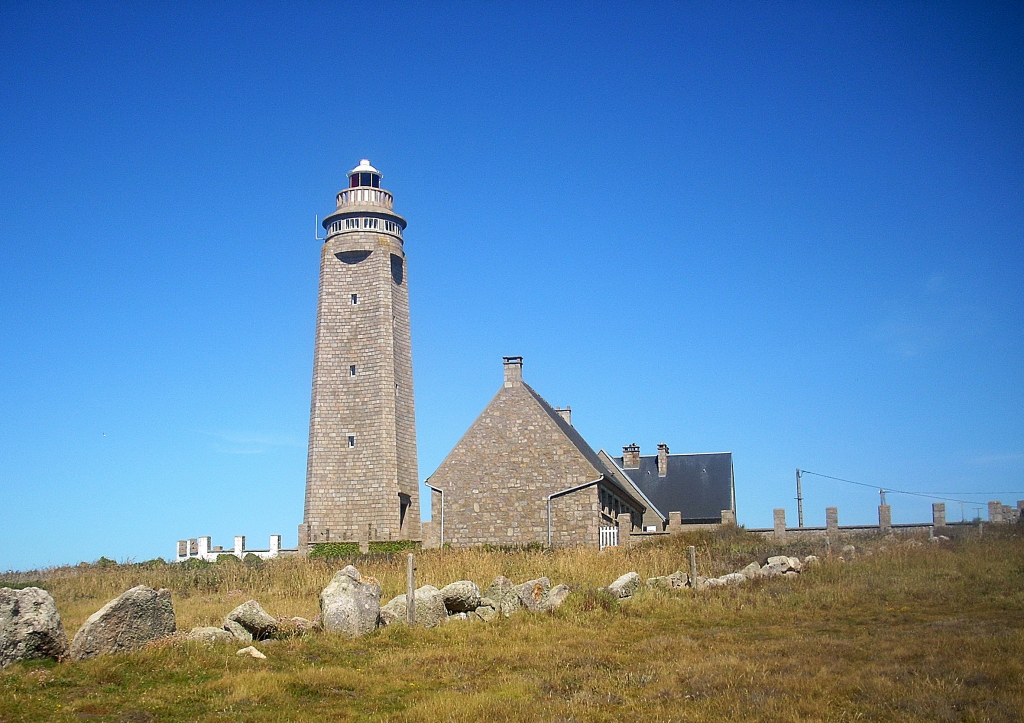
\includegraphics[width=9cm]{./test02.png}
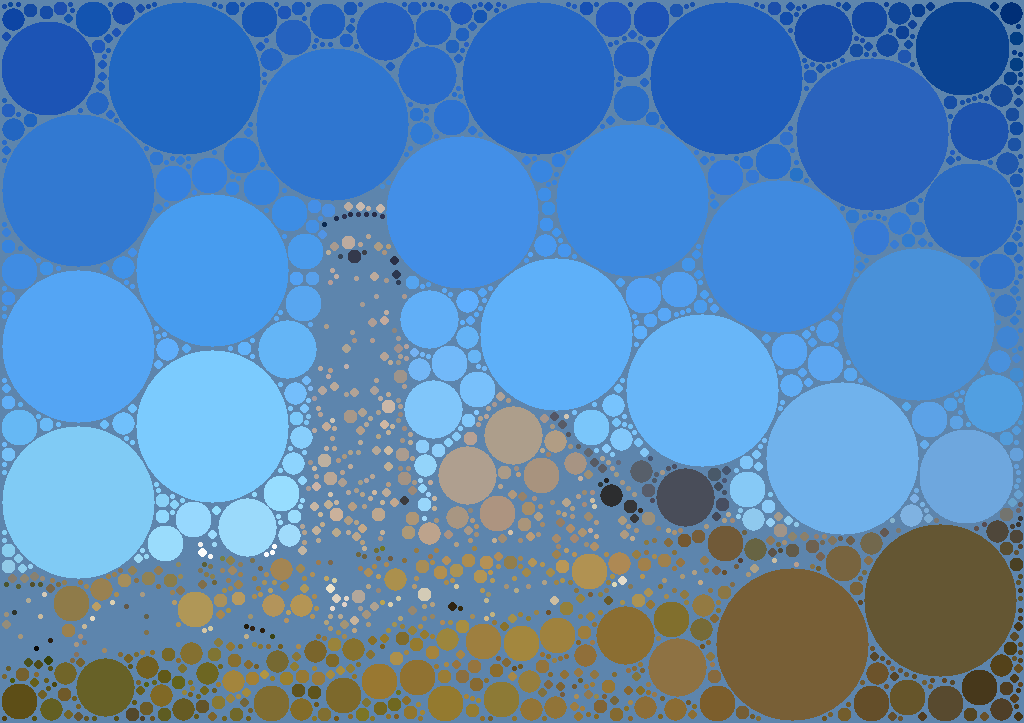
\includegraphics[width=9cm]{./out02.png}
\end{figure}
\end{center}

\begin{center}
\begin{figure}[H]
\centering
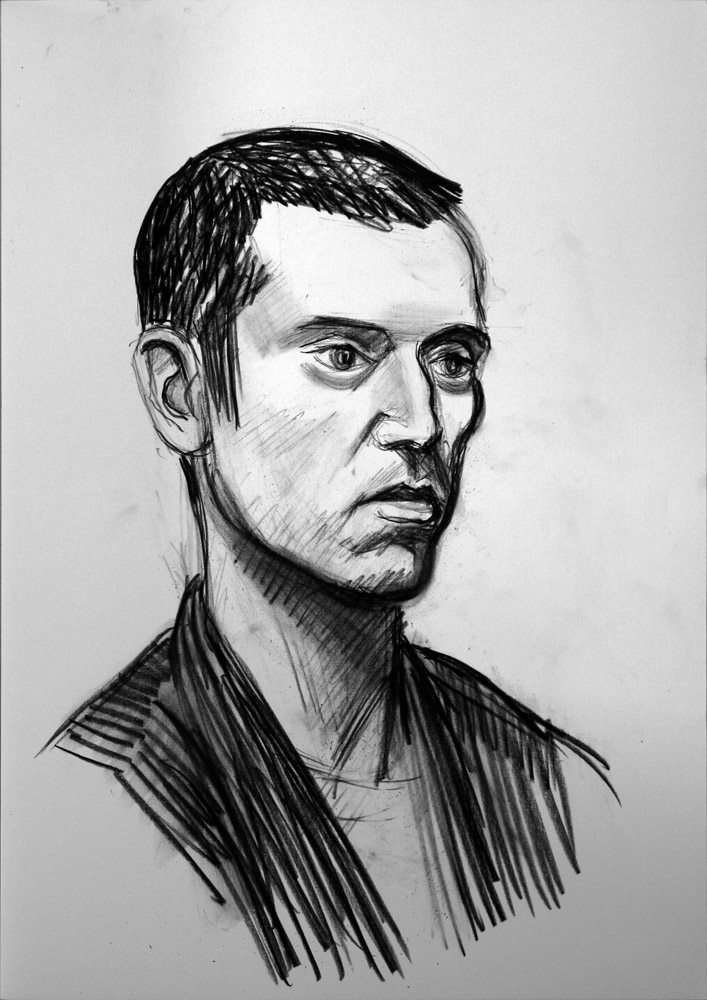
\includegraphics[width=7cm]{./test05.png}
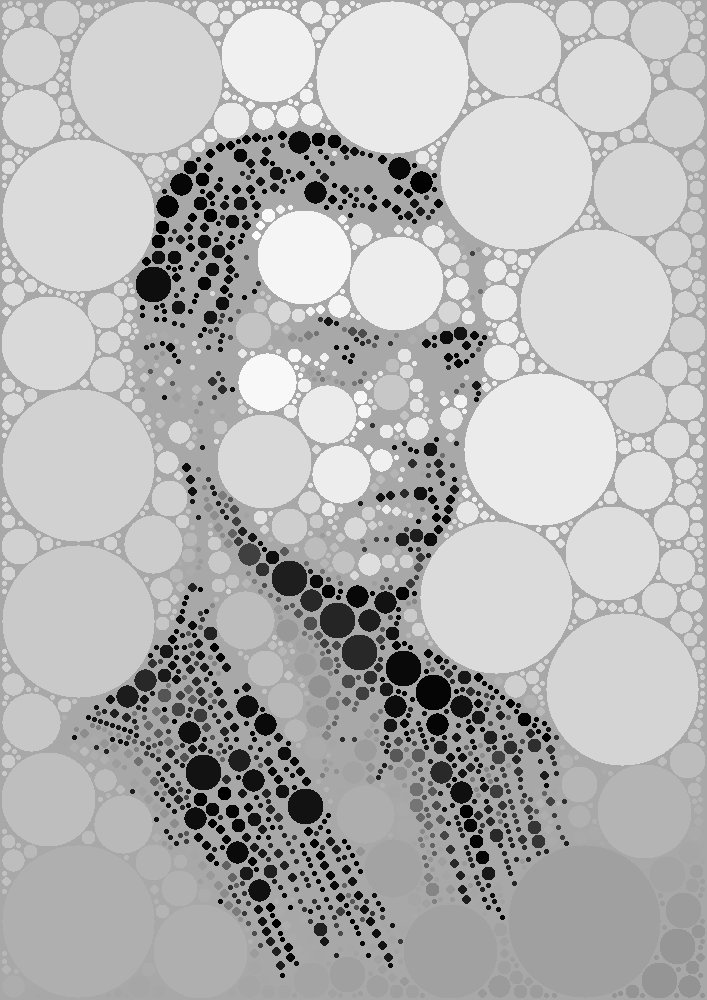
\includegraphics[width=7cm]{./out05.png}
\end{figure}
\end{center}

\end{document}


